\section{Work Done}
  In this next section I will discuss the work that was carried on the project. In our team we have \textit{'ways of working'}
  flowchart that helps guides us in how the project should be done throughout the team (GoRetro, 2023). Our ways of working is broken down into 5 sections, 
  all of which will be discussed. For a full diagram of our workflow see \hyperref[sec:AppendixD]{\textbf{Appendix D}}.

  \subsection{Requirements and epic creation}

  \begin{figure}[H]
    \centering
    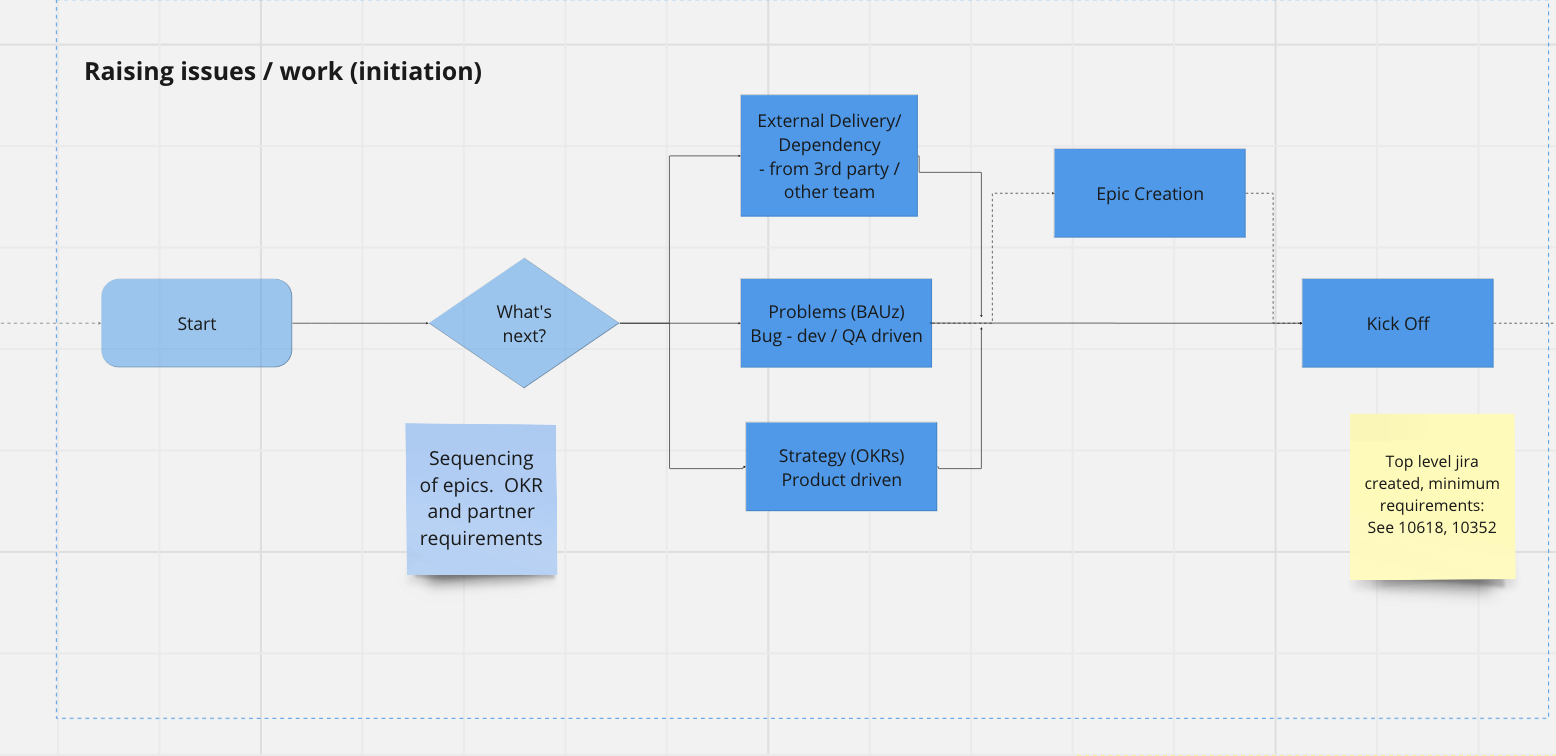
\includegraphics[width=8cm]{assets/workflow/initiate.png}
    \caption{Initiation stage of for ways of working.}
    \label{fig:workflowInitiate}
  \end{figure}

  \subsection{Investigation and spike}

  \begin{figure}[H]
    \centering
    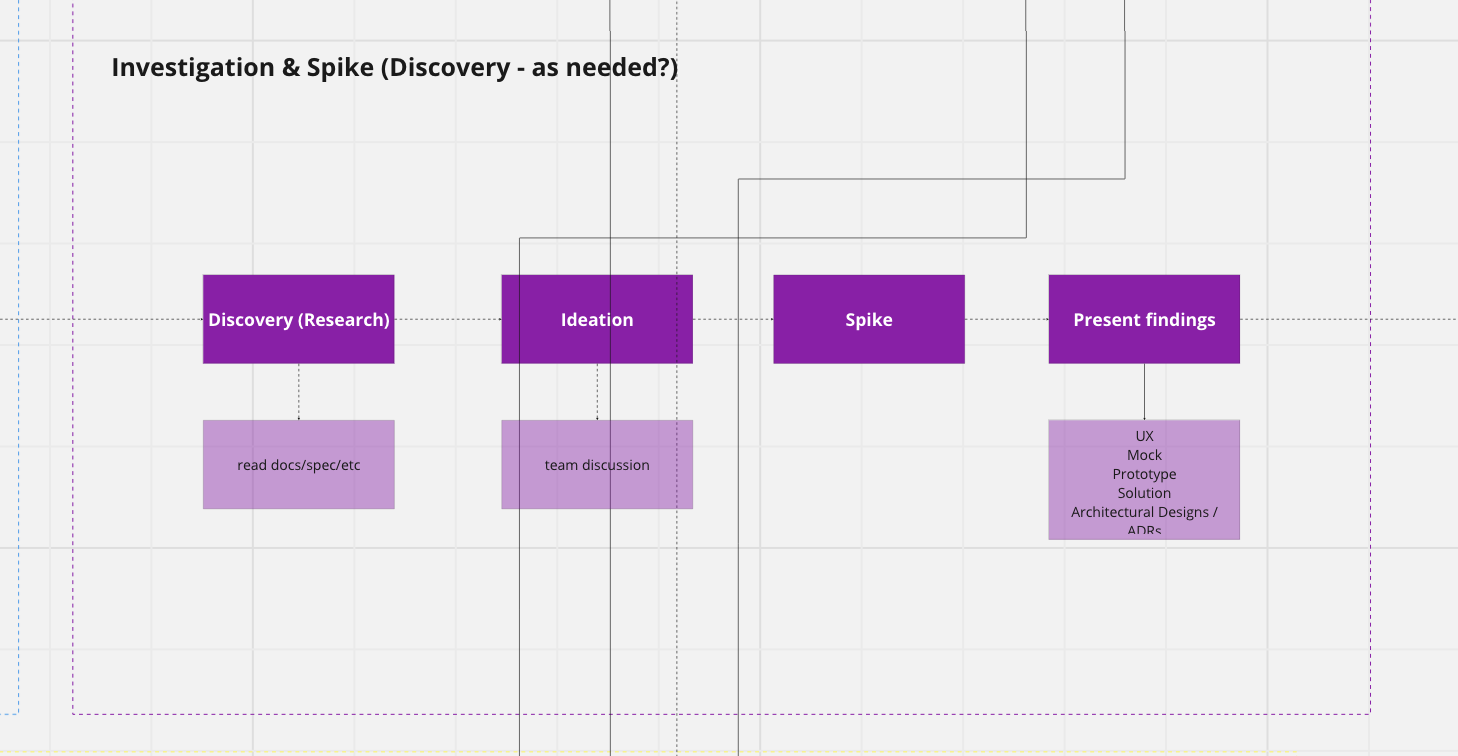
\includegraphics[width=8cm]{assets/workflow/investigation.png}
    \caption{Investigation stage of for ways of working.}
    \label{fig:workflowInvestigation}
  \end{figure}

  \subsection{Slicing and kick-off}

  \begin{figure}[H]
    \centering
    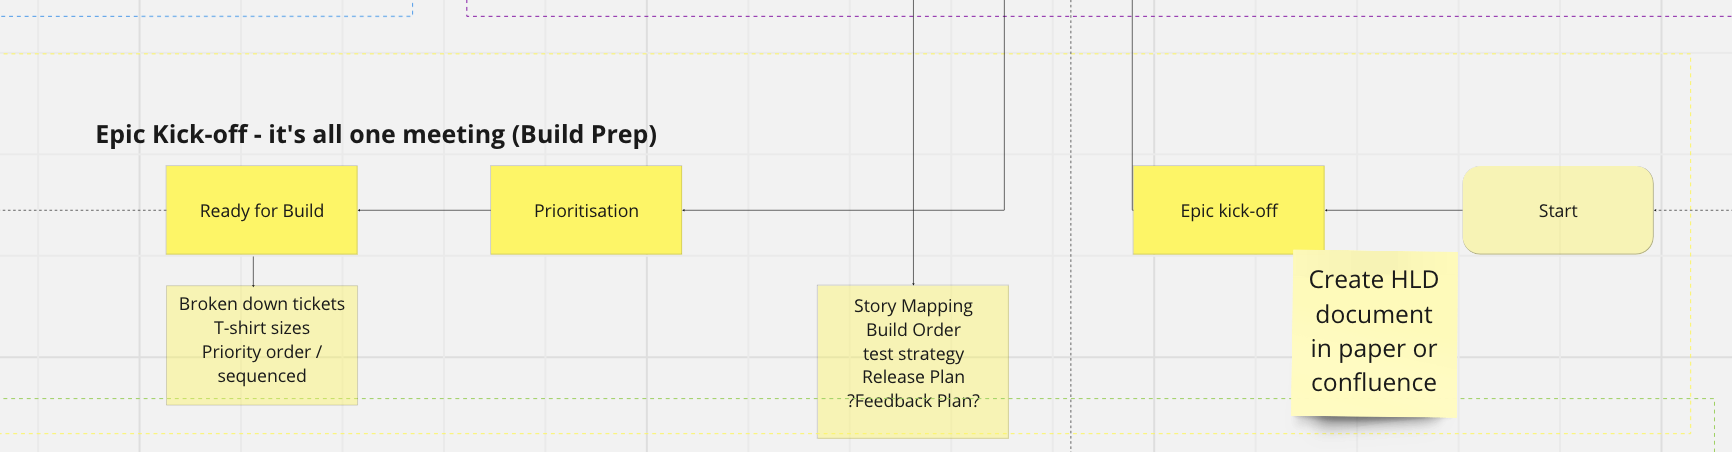
\includegraphics[width=8cm]{assets/workflow/kickoff.png}
    \caption{Kick-off stage of for ways of working.}
    \label{fig:workflowKickOff}
  \end{figure}

  \subsection{Build software}

  \begin{figure}[H]
    \centering
    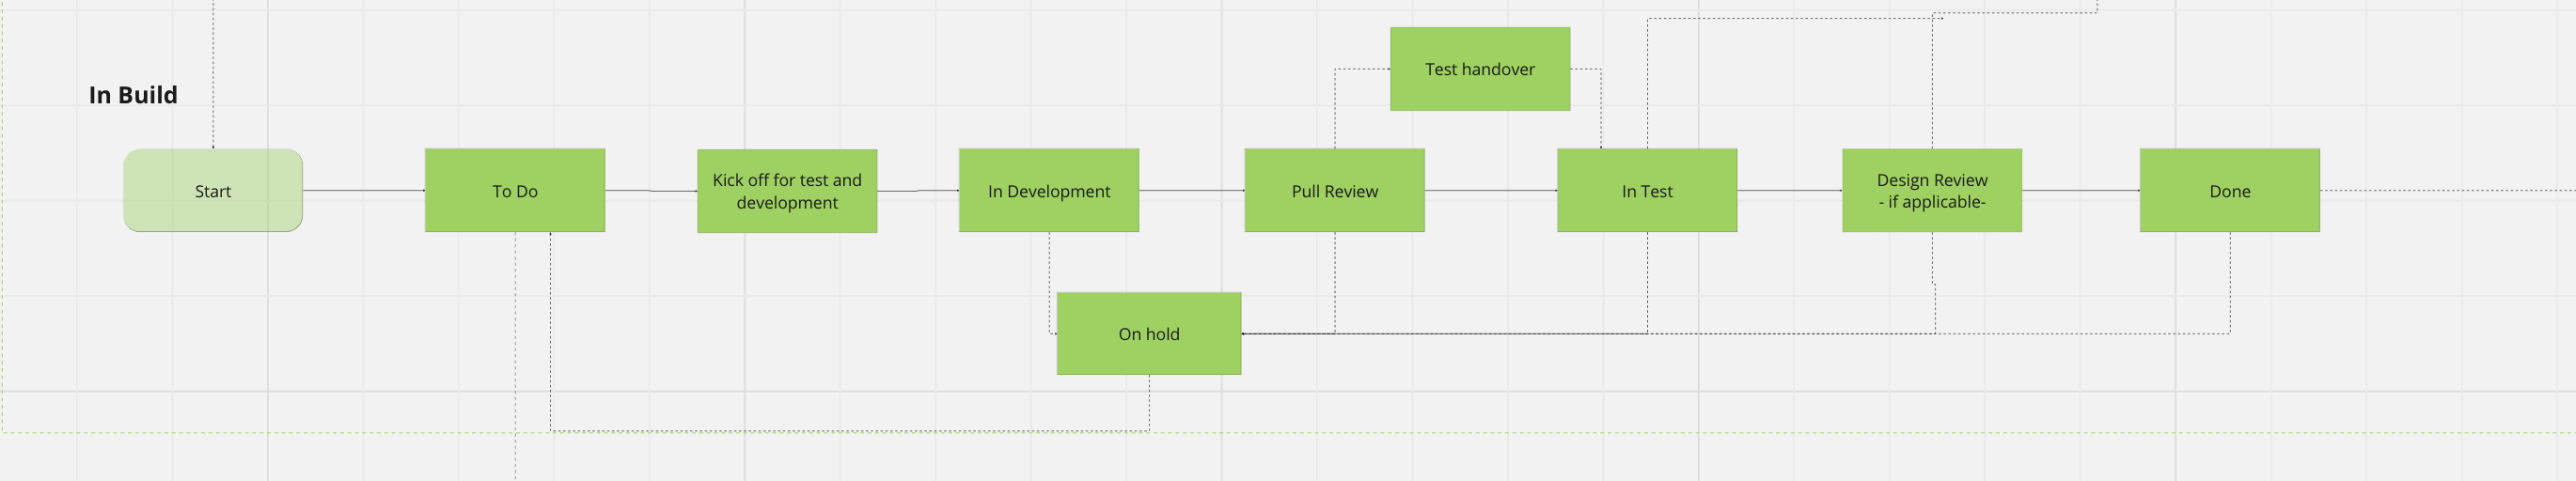
\includegraphics[width=8cm]{assets/workflow/build.png}
    \caption{Build stage of for ways of working.}
    \label{fig:workflowBuild}
  \end{figure}

  \subsection{Release}

  \begin{figure}[H]
    \centering
    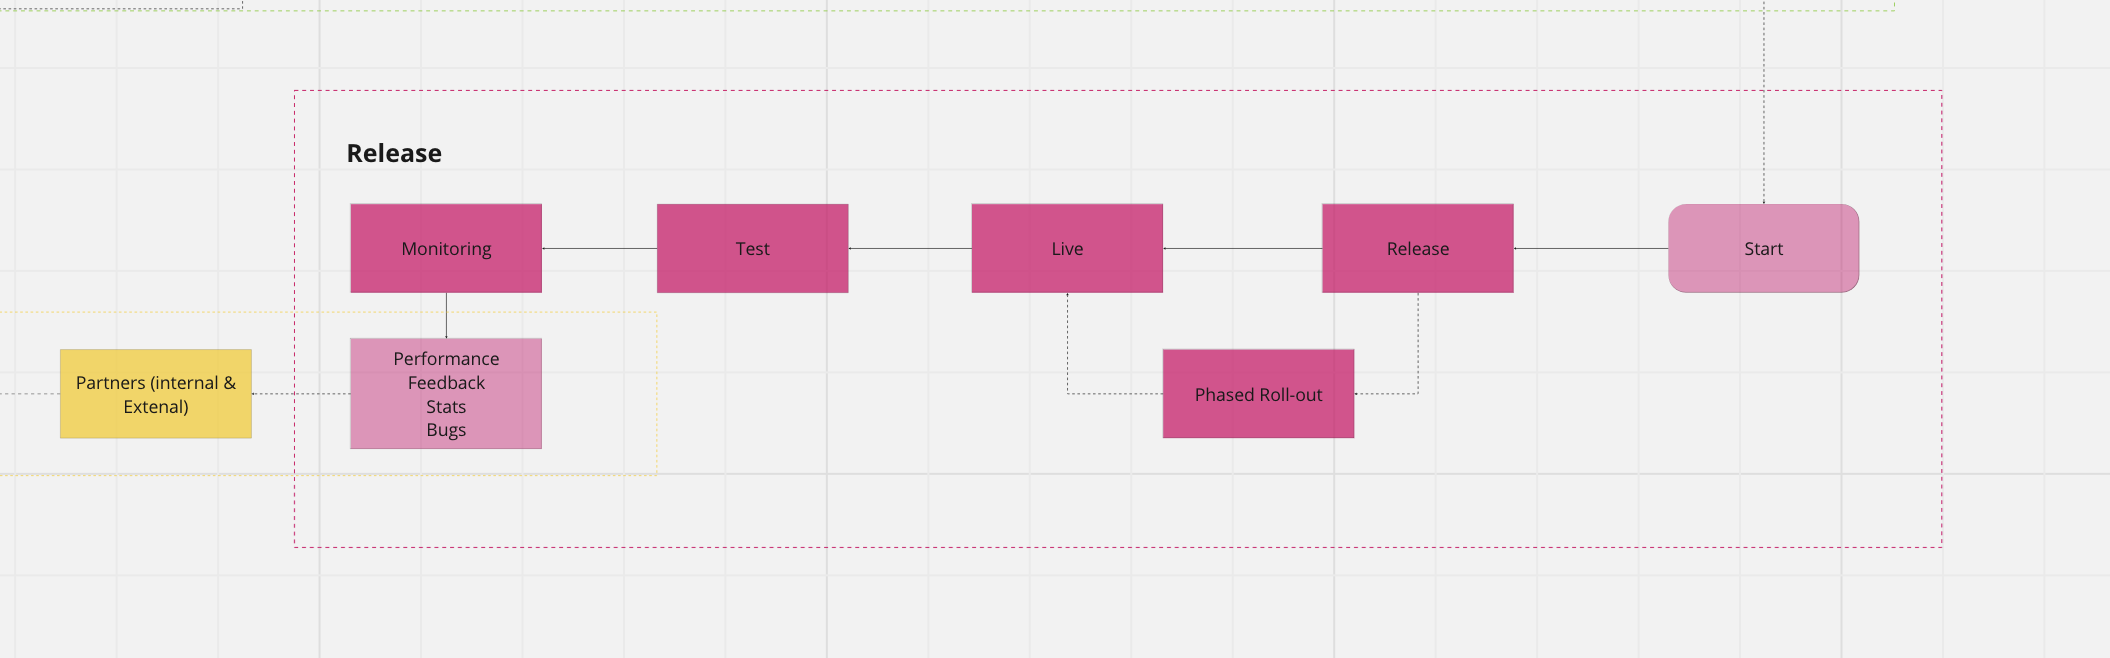
\includegraphics[width=8cm]{assets/workflow/release.png}
    \caption{Release stage of for ways of working.}
    \label{fig:workRelease}
  \end{figure}

\newpage
